\chapter{Enzyme Kinetics} \label{ch:enzyme}

\section{Fast and Slow Dynamics}

Suppose we are modeling a system in which some states, call them $z$
more very quickly to some equilibrium value. Meanwhile other states,
call them $x$, change more slowly. In equations, we write
%
\begin{eqnarray}
\dot x & = & f ( x, z, t, \epsilon ) \label{eqn:fast-slow1} \\
\epsilon z & = & g ( x, z, t, \epsilon ). \label{eqn:fast-slow2}
\end{eqnarray}
%
Here, $\epsilon$ denotes some system parameter (such as a reaction
rate), that is very small compared with other parameters. You can see
that if you divide \eref{eqn:fast-slow2} by $\epsilon$ then the rate
of change of $z$ is, thus, large. 

Since $\epsilon$ is small, we might as well ask what if
$\epsilon=0$. In this case, \eref{eqn:fast-slow2} becomes
%
\begin{equation} \label{eqn:fast-slow-eqality}
g ( x, z, t, 0 ) = 0. 
\end{equation}
%
Suppose that $z=h(x,t)$ is a solution to
\eref{eqn:fast-slow-equality}. Then the ``slow dynamics'' of $x$ are
described by
%
\begin{equation} \label{eqn:fast-slow-reduced}
\dot x = f ( x, h(t,x), t, 0 ), 
\end{equation}
%
that is, solely in terms of $x$. Thus, by assuming that $\epsilon=0$,
we have come up with a reduced model of the original system. It turns
out that how much smaller $\epsilon$ is compared to other parameters
in the system determines the degree to which the full and reduced
models are similar.

\section{Enzyme Reactions}

\subsection{The Michaelis-Menten Model}

As an example, consider the reaction
%
$$
E + S \xrightleftharpoons[\text{$k_2$}]{\text{$k_1$}} ES \xrightharpoon[\text{}]{\text{$k_3$}} E + P
$$
%
which describes how a species of enzyme $E$ interacts with a substrate
species $S$ to produce a product species $P$. An enzyme molecule may repeatedly
bind to substrate molecules to form enzyme-substrate complexes
$ES$. Eventually the enzyme turns the a substrate molecule into a
product. It is often the case that
$$
k_1, k_2 \gg k_3, 
$$
suggesting that the population of $ES$ stabilizes quickly compared to
the production of $P$. 

\begin{figure}
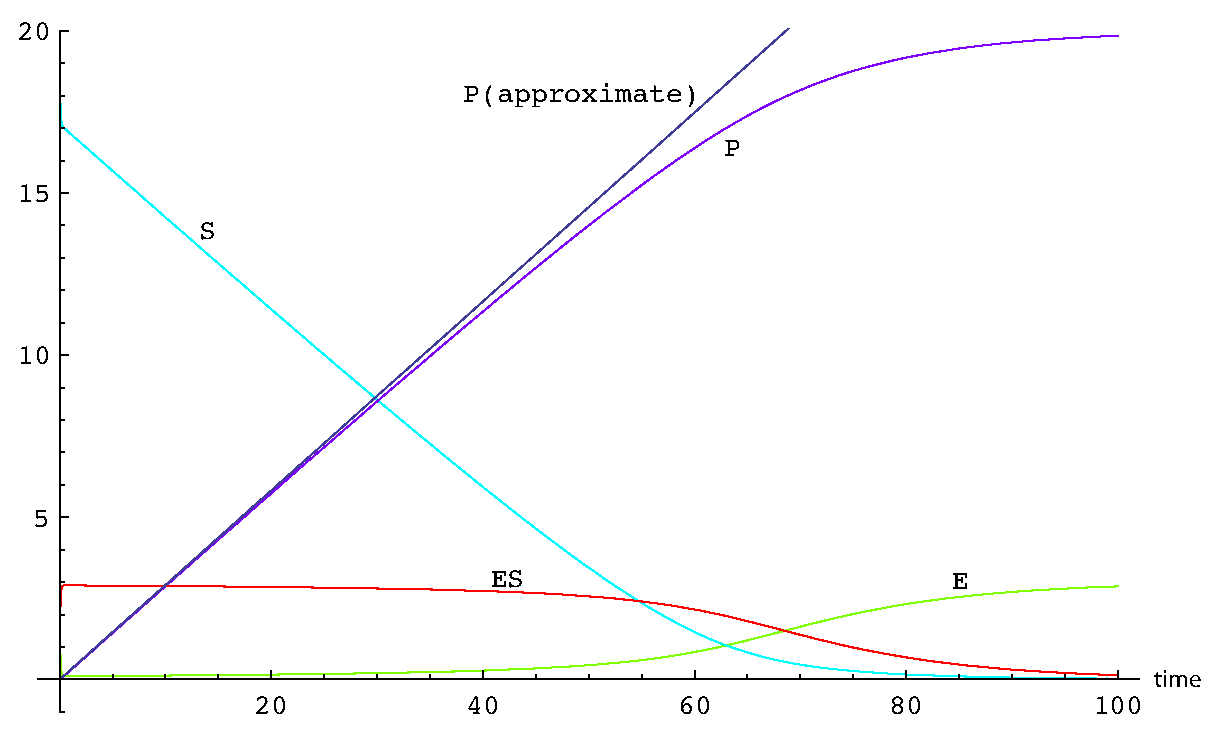
\epsfig{file=figures/michaelis-menton.eps, scale=0.6}
  \caption{\label{fig:mm} The simple enzyme substrate reaction and the
    Michaelis-Menton approximation. Here, $k_1=1.0$, $k_2=0.5$,
    $k_3=0.1$, $v_E(0)=3$ and $v_S(0)=20$.}
\end{figure}

Now consider the analysis question: at approximately what rate is $P$
produced, ignoring the brief period of time during which $ES$ is
equilibrating? Treating $v_S$ as a constant (i.e. assuming there are a
very large number of substrate molecules), and using the law of mass
action gives
\begin{eqnarray}
\dot v_{P}  & = & k_3 v_{ES} \\
\dot v_{ES} & = & k_1 v_E v_s - k_2 v_{ES} - k_3 v_{ES} .
\end{eqnarray}
The total amount of enzyme does not change so that $v_E + v_{ES} =
E_{tot}$. Thus, the equation for $\dot v_E$ is not needed and
%
\begin{eqnarray*}
\dot v_{ES} & = & k_1 (E_{tot}-v_{ES}) v_s - k_2 v_{ES} - k_3 v_{ES} \\
           & = & k_1 e_{tot} v_s - (k_1 s + k_2 + k_3 ) v_{es} .
\end{eqnarray*}
%
Now define $\epsilon \defeq (k_1 v_s + k_2 + k_3)^{-1}$. By our assumptions
on the relative magnitudes of the $k_i$ and that $s$ is large, it
follows that $\epsilon$ is small. We can now write:
%
\begin{eqnarray}
\dot v_{P}  & = & k_3 v_{ES} \label{eqn:mm-sv1} \\
\epsilon \dot v_{ES} & = & \frac{k_1 e_{tot} v_s}{k_1 v_s + k_2 + k_3} - v_{es},  \label{eqn:mm-svp2}
\end{eqnarray}
%
which matches \eref{eqn:fast-slow1} and \eref{eqn:fast-slow2}. Setting
the fast dynamics to zero gives the constraint that
%
$$
v_{es} = \frac{k_1 e_{tot} v_s}{k_1 s + k_2 + k_3}
$$
%
and substituting into \eref{eqn:mm-sv1} gives
%
$$
\dot v_{P} = \frac{k_3 k_1 e_{tot} v_s}{k_1 v_s + k_2 + k_3} = \frac{k_3 e_{tot} v_s}{v_s + \frac{k_2+k_3}{k_1}}.
$$
Chemists and biologists like to define
%
$$
V_{max} \defeq k_3 e_{tot} \;\;\;\;\; K_m = \frac{k_2+k_3}{k_1}
$$
%
so that we arrive at the {\em Michaelis-Menton} model:
%
\begin{equation} \label{eqn:mm}
\dot v_{P} = \frac{V_{max} v_s}{v_s+K_m}.
\end{equation}
%
The constant $V_{max}$ is commonly referred to as the maximum
production rate, which you get when $v_s \rightarrow \infty$. The
constant $K_m$ is called the half saturation constant, which is the
concentration of $S$ required to get a rate of $V_{max}/2$. 

The situation is shown in Figure~\ref{fig:mm}. Initially, while the
amount of substrate is high, the rate of change of $P$ is essentially
constant with slope defined by Equation~\eref{eqn:mm}. Eventually, the
substrate is depleted, and the assumption that $\dot v_S = 0$ no
longer holds.

\subsection{Competetive Inhibition}

Now consider a system consisting of an enzyme in one of two states,
either active $E$ or bound to a deactivator $I$ to form an inactive
complex $EI$. The reactions are
$$
E + S \xrightleftharpoons[\text{$k_{-1}$}]{\text{$k_1$}} ES \xrightharpoon[\text{}]{\text{$k_2$}} E + P
$$
$$
E + I \xrightleftharpoons[\text{$k_{-3}$}]{\text{$k_3$}} EI .
$$
In this case, we say that $I$ and $S$ are in competition for $E$. If
$ES$ and $EI$ equilibrate quickly, then it seems reasonable to
approximate the system by a simple one dimensional system in which the
product $P$ is produced at some rate that is a function of the
concentrations of $S$ (which we'll assume is large and relatively
unchanging) and $I$ (which is not produced or consumed). 

First, note that there we have the conservation constraint that the
enzyme is either free, bound to an $S$ or bount to an $I$. That is, 
%%
$$
v_{tot} = v_E + v_{ES} + v_{EI}. 
$$
%%
Assuming that $ES$ and $EI$ equilibrate quickly gives
$$
\dot v_{ES} = 0 = k_1 v_E v_S - (k_{-1}+k_2)v_{ES}
$$
%%
so that $v_Ev_S = K_m v_{ES}$ where $K_m = ( k_{-1}+k_2 ) / k_1$ and
$$
\dot v_{EI} = 0 = k_3 v_E v_I - k_{-3} v_{EI}
$$
which implies that $v_E v_I = K_3 v_{EI}$ where $K_3 =
\frac{k_{-3}}{k_{3}}$. Putting these relationships into the constraint
above gives
%
\begin{eqnarray*}
v_{tot} & = & \frac{K_m v_{ES}}{v_S} + \frac{v_Ev_I}{K_3} + v_{ES} \\
       & = & \frac{K_mv_{ES}}{v_S} + \frac{K_mv_{ES}}{v_S} \frac{v_I}{K_3} + v_{ES}
\end{eqnarray*}
%
which implies that 
%
$$
v_{ES} = \frac{v_{tot}}{\frac{\displaystyle K_m}{\displaystyle v_S} + \frac{\displaystyle K_m v_I}{\displaystyle K_3v_S} + 1}
       = \frac{v_{tot}v_S}{K_m + \frac{\displaystyle K_m}{\displaystyle K_3}v_I + v_S} .
$$
%
From the above expression for $v_{ES}$ it follows that
%
\begin{equation}
\dot v_P \approx \frac{V_{max} v_S}{K_m + \frac{\displaystyle K_m}{\displaystyle K_3} v_I + v_S}
\end{equation}
%%
where 
%%
$$
V_{max} = k_2 v_{tot} \;\;\;\; K_m = \frac{k_{-1}+k_2}{k_3} \;\;\;\; \mathrm{and} \;\;\; K_3 = \frac{k_{-3}}{k_3}. 
$$
If there is no inhibitor $I$, we get the same results as with the
Michaelis-Menton system. As the concentration of $I$ increases, the
rate of production of $P$ goes to zero. Finally, if there is a high
concentration of $S$, then $\dot v_P \approx V_{max}$. The situation
is shown in Figure~\ref{fig:comp-inhibit} \enx
%%

\begin{figure}
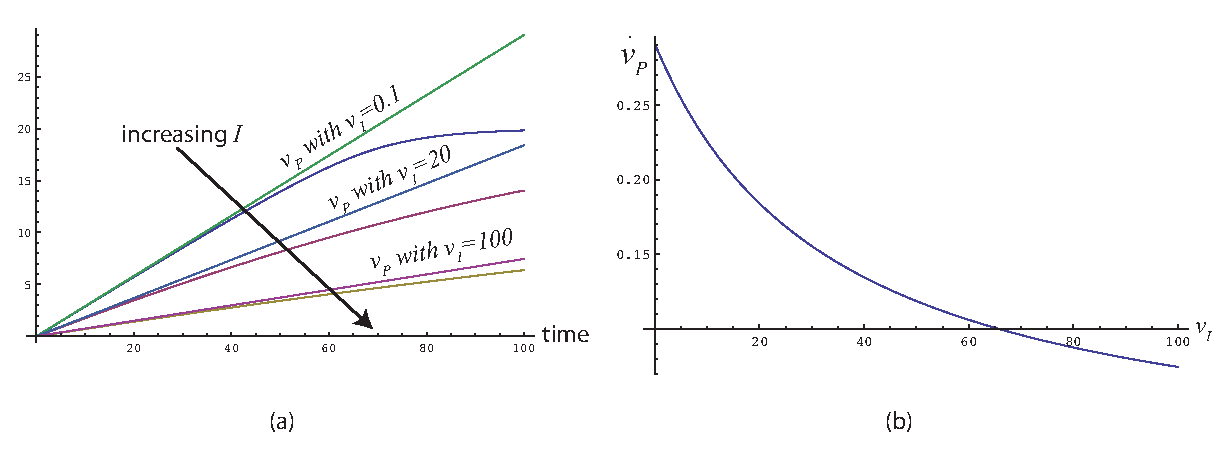
\epsfig{file=figures/comp-inhibit-together.eps, scale=0.65}
\caption{\label{fig:comp-inhibit} The competitive inhbition model. (a)
  Three different values for $v_I$ and the resulting dynamics for
  $v_P$ both the exact models (curves) and approximations (striaght
  lines). (b) As $v_I$ increases, the rate of production of $P$
  decreases.  }
\end{figure}


\section{Hill Functions}

Models of genetic regulatory networks can get big fast, in terms of
the number of species, the number of reactions, and the number of
unknown parameters. One way to reduce this complexity slightly is to
assume that regulatory interactions, such as the binding and unbinding
of a repressor to the regulatory region of a gene, are much faster than
the transcription and translation reactions. In fact, this is usually
a pretty safe assumption, although one has to be careful. The result
is to write rate of production of a gene's product in terms of the
{\em fraction} of action versus total gene:
%
\begin{equation} \label{eqn:gene-fraction}
\dot X = \alpha \frac{g_\mathrm{active}}{g_\mathrm{total}} + \alpha_0 - \beta X
\end{equation}
%
where $\alpha$ is the maximum rate of production, $\alpha_0$ is the
rate of ``leaky'' expression (sometimes used in these models, although
not strickly legitimate), and $\beta$ is the rate of protein
degradation and dilution. 

\begin{example}
Consider a gene $g$ repressed by a transcription factor $R$ via the following reaction
%
$$
g_\mathrm{on} + nR \xrightleftharpoons[\text{$k_{r}$}]{\text{$k_f$}} g_\mathrm{off} . 
$$
The number $n$, called the {\em cooperativity}, is the number of
molecules of $R$ that must bind to $g$ to turn it off. The reaction is
a bit unrealistic, as the likelihood that $n+1$ molecules
simultaneously interact and react is low for $n>1$. The idea is that
the reaction above is actually implemented by the sequential or
parallel binding of individual molecules $R$, one after the other. The
details of how different mechanisms affect the results in this example
are explored in the exercises (and see also \cite{hill-misuse}). 

\begin{figure}
\epsfig{file=figures/hill.eps, scale=0.8}
\caption{\label{fig:hill-repress} The Hill Function
  (Equation~\eref{eqn:hill-repress}) for repression plotted for
  various values of the cooperativity $n$. The function essentially
  computes the Boolean function $\neg R$. That is, when $R$ is not
  present, the gene is expressed. Otherwise it is not expressed.}
\end{figure}

If we assume that $k_r$ and $k_f$ are large, then, at equilibrium, we get
%%
$$
k_f g_\mathrm{on} R^n = k_r g_\mathrm{off} . 
$$
%%
Thus,
\begin{equation}\label{eq:hill-repress}
\frac{g_\mathrm{on}}{g_\mathrm{on}+g_\mathrm{off}} = 
  \frac{g_\mathrm{on}}{g_\mathrm{on}+\frac{k_f g_\mathrm{on} R^n}{k_r}} = \frac{1}{1+\frac{R^n}{K_\mathrm{eq}}} 
\end{equation}
where $K_\mathrm{eq} = k_r / k_b$ is the equilibrium constant of the
reaction. The result is a so called {\em Hill Function}
\cite{hill-function-1910} and is plotted in
Figure~\ref{fig:hill-repress} for various values of $n$. The Hill
function for repression inserted into
Equation~\eref{eqn:gene-fraction} results in 
%
$$
\dot X =  \frac{\alpha}{1+\frac{R^n}{K_\mathrm{eq}}}  + \alpha_0 - \beta X ,
$$
%
which describes the rate of production of a protein $X$ given the
concentration of the repressor $R$. This system essentially
  computes the Boolean function $\neg R$. That is, when $R$ is not
  present, the gene is expressed. Otherwise it is not expressed. \enx
\end{example}

\begin{example}
A similar function for activation can be obtained by considering the reactions
%
$$
g_\mathrm{off} + n A \xrightleftharpoons[\text{$k_{r}$}]{\text{$k_f$}} g_\mathrm{on} . 
$$
%
which results in the activation Hill Function
%
$$
\frac{g_\mathrm{on}}{g_\mathrm{on}+g_\mathrm{off}} = \frac{K_\mathrm{eq}A^n}{A^n + K_\mathrm{eq}},
$$
%
which can be substituted into Equation~\eref{eqn:gene-fraction} to
obtain a model for the production of a gene product as a function of
the activator concentration. 
%
\enx
\end{example}

\begin{figure}
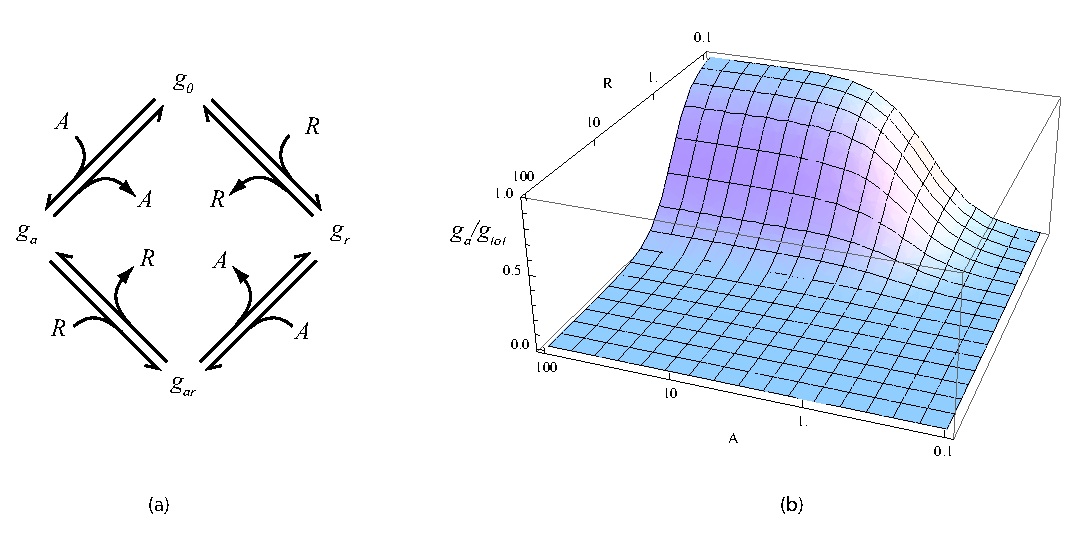
\epsfig{file=figures/act-rep.eps, scale=0.8}
\caption{\label{fig:act-rep} The Hill Function
  (Equation~\eref{eqn:alt-rep}) for a gene that is activated by a
  transcription factor $A$ and repressed by a transcription factor
  $R$.  The Hill function essentially computes the Boolean function $A
  \wedge \neg R$.  }
\end{figure}

\begin{example} (THERE ARE A BUNCH OF ERRORS IN THIS EXAMPLE TO BE
  FIXED) Many genes are regulated by several transcription factors,
  some that are activators, some that are inhibitors. Hill functions
  can be devised to model such situations as well. Here is an
  example. Suppose that a gene can be in one of four states: (1) $g_0$
  with no transcriptions factors bound; (2) $g_a$ with an activator
  bound; (3) $g_r$ with a repressor bound; (4) and $g_{ar}$ with both
  an activator and a repressor bound. The reaction network is shown in
  Figure~\ref{fig:act-rep}(a). At equilibrium, we have
%
\begin{eqnarray*}
k_1 g_0 & = & k_{-1} g_a \\
k_2 g_0 & = & k_{-2} g_r \\
k_3 g_a & = & k_{-3} g_{ar} \\
k_4 g_r & = & k_{-4} g_{ar} .
\end{eqnarray*}
Thus, the total amount of gene in the system is
%
\begin{eqnarray*}
g_\mathrm{tot} & = & g_0 + g_a + g_r + g_{ar} \\
 & = & g_0 + K_1 g_0 A^n + K_2 g_0 R^m + K_3 g_a R^m \\
 & = & g_0 + K_1 g_0 A^n + K_2 g_0 R^m + K_3  K_1 g_0 A^n R^m 
\end{eqnarray*}
where $K_i = k_i / k_{-i}$. From the above expression we obtain the Hill Function 
%
\begin{equation}\label{eq:alt-rep}
\frac{g_a}{g_\mathrm{tot}} = \frac{K_1 A^n}{1 + K_1A^n + K_2R^m + K_3  K_1A^n R^m}.
\end{equation}
%
This function is plotted for $m=n=2$ and $K_i=1$ in
Figure~\ref{fig:act-rep}(b). Only when the concentration of $A$ is
high and the concentration of $R$ is low is the gene active. In
logical terms, the system implements the Boolean function $A \wedge \neg R$. 
%
\enx
\end{example}

Warning: The cooperativity $n$ is a subject of some debate and
misuse. It is not unusual to find a paper stating that, for their
system, $n$ is not an integer! The reason is that Hill Functions are
used more to {\em fit} data than they are as first-principles models
like we are presenting them above. The student is warned to treat the
parameter $n$ with a grain of salt: It does not necessarily correspond
to anything physical. In fact, relieved of the need for a physical
meaning for $n$, we are free to treat it as just another parameter.




\section{Problems}

\setcounter{exercount}{0}

\begin{exercise}
Consider the system
%
$$
EA + S \xrightleftharpoons[\text{$k_{-1}$}]{\text{$k_1$}} EAS \xrightharpoon[\text{}]{\text{$k_2$}} EA + P
$$
$$
E + A \xrightleftharpoons[\text{$k_{-3}$}]{\text{$k_3$}} EA .
$$
%
in which an enzyme has an inactive form $E$ and an active form
$EA$. The molecule $A$ in this system is an activator. Determine an
enzyme kinetics model for this system similar to the competive
inhibition. That is, determine an approximate rate of product
production as a function of $v_S$ and $v_A$. Compare the mass action
kinetics model of the system with the appoximate version in simulation
to produce a plot similar to that in Figure~\ref{fig:comp-inhibit}(a).
\end{exercise}

\begin{exercise}
  Determine the Hill Function for the case of two activators where the
  active state of the gene is when both activators are bound to the gene.
\end{exercise}

\begin{exercise}
Consider the bistable switch described by
%
\begin{eqnarray*}
2A_1 & \rreact{k_1}{u_1} &  B_1  \\
2A_2 & \rreact{k_2}{u_2} &  B_2  \\
g_1 + B_2 & \rreact{\gamma_1}{\gamma_2} & g_{1,\mathit{off}} \\
g_2 + B_1 & \rreact{\gamma_1}{\gamma_2} & g_{2,\mathit{off}} \\
g_i & \react{\alpha} g_i + A_i \\
A_i & \react{\beta} & \varnothing
\end{eqnarray*}
%
Find equations for this system. Find two conservations and use them to
reduce the number of equations by two. Assume that the first four
reactions are fast and use the resulting equalities reduce the
equations further.
\end{exercise}